\chapter{Fault Detection}

Fault detection deals with detecting system discrepancies, abnormal behaviour. It is the first step towards handling faults. It doesn't necessarily identify the source of the fault, just establishes the fact that a fault has occurred in the system.


\section{Motors fault detection}

\label{sec:structural}
\subsection{Structural Analysis}
Structural analysis studies the interrelation between parameters and variables of the system using constraints between them. It distinguishes known and unknown variables, according to whether they can be measured in the system or not. Then the unknown variables are expressed using the known ones according to the constraints. Structural analysis based residual signal require that unknown variables can be expressed redundantly. One of the constraints is used to express the unknown, the other to verify it. If there's a mismatch between the two, a fault is detected.

In case of fault detection in sensors, one constraint is between the measured and the actual values of a variable. In case of a sensor fault, there can be a considerable difference between the measured and the actual value of a variable.

Assumes that only one fault occurs at any given time, so faults cannot mutually neutralize each other. 

The constraints being used to detect faults in the motor are:

\ref{sec:motor} \todo{reference motor section properly}


\begin{equation}
V_a = R_a * i + k_e \omega
\end{equation}

$L_a$ is negligible

\begin{equation}
 k_{t}i  =J\dfrac{d\omega}{dt} + b\omega
\end{equation}

\begin{equation}
\tau = k_t i
\end{equation}

$d_1(\omega, \dot{\omega})$


\subsection{Alternative method for identifying reaction wheel fault}

With enough computational power the faulty reaction wheel can be detected through the calculated reaction wheel output torque, assuming only one reaction wheel is faulty. It is done by calculating the difference between 3D torque demand and actual 3D torque output. 

\begin{equation}
\vec{N}_{rw} = \underline{I}_s \dot{\vec{\omega}}  + \vec{\omega} \times \vec{h_{rw}} - \vec{N_{mt}} - \vec{N_{dist}}
\end{equation}

Then the difference between torque demand and torque output is calculated. The reaction wheel that has the most similar axis orientation to the torque difference is deemed as faulty.

\begin{equation}
\vec{N}_{rw}^{demand} - \vec{N}_{rw}^{actual} = 
\vec{N}_{rw}^{diff}
\end{equation}

\begin{equation}
 \pm \vec{N}_{rw}^{diff}  \stackrel{?}{\approx} \vec{axis} 
\end{equation}


\todo{mention unit vector notation, decide notation for axis, express axis according to q}

Note: the lag for torque change and wheel saturation has to be taken into account separately, as those don't count as faults. 
Thresholds should be applied.

\section{Magneto torquers  fault detection}

\subsection{Unknown Input Observer (UIO)}

Uncertainties and modeling errors may cause discrepancies between the actual system and the descriptor mathematical model. Linearization and simplifications which make the system more manageable may lead also to uncertainties. All these uncertainties can have an effect on the system dynamic behavior through the input signals.   
A residual, fault indicator, based on observer design can be robust regarding the unknown input signals by making the effect of unknown inputs(UI) insensitive to the residual and thus making possible to maximize the detectability of a fault. 
Following \cite{UIO}     
\section{Motors fault detection}

\label{sec:structural}
\subsection{Structural Analysis}
Structural analysis studies the interrelation between parameters and variables of the system using constraints between them. It distinguishes known and unknown variables, according to whether they can be measured in the system or not. Then the unknown variables are expressed using the known ones according to the constraints. Structural analysis based residual signal require that unknown variables can be expressed redundantly. One of the constraints is used to express the unknown, the other to verify it. If there's a mismatch between the two, a fault is detected.

In case of fault detection in sensors, one constraint is between the measured and the actual values of a variable. In case of a sensor fault, there can be a considerable difference between the measured and the actual value of a variable.

Assumes that only one fault occurs at any given time, so faults cannot mutually neutralize each other. 

The constraints being used to detect faults in the motor are:

\ref{sec:motor} \todo{reference motor section properly}


\begin{equation}
V_a = R_a * i + k_e \omega
\end{equation}

$L_a$ is negligible

\begin{equation}
k_{t}i  =J\dfrac{d\omega}{dt} + b\omega
\end{equation}

\begin{equation}
\tau = k_t i
\end{equation}

$d_1(\omega, \dot{\omega})$


\subsection{Alternative method for identifying reaction wheel fault}

With enough computational power the faulty reaction wheel can be detected through the calculated reaction wheel output torque, assuming only one reaction wheel is faulty. It is done by calculating the difference between 3D torque demand and actual 3D torque output. 

\begin{equation}
\vec{N}_{rw} = \underline{I}_s \dot{\vec{\omega}}  + \vec{\omega} \times \vec{h_{rw}} - \vec{N_{mt}} - \vec{N_{dist}}
\end{equation}

Then the difference between torque demand and torque output is calculated. The reaction wheel that has the most similar axis orientation to the torque difference is deemed as faulty.

\begin{equation}
\vec{N}_{rw}^{demand} - \vec{N}_{rw}^{actual} = 
\vec{N}_{rw}^{diff}
\end{equation}

\begin{equation}
\pm \vec{N}_{rw}^{diff}  \stackrel{?}{\approx} \vec{axis} 
\end{equation}


\todo{mention unit vector notation, decide notation for axis, express axis according to q}

Note: the lag for torque change and wheel saturation has to be taken into account separately, as those don't count as faults. 
Thresholds should be applied.

\section{Magneto torquers  fault detection}
\subsection{Unknown Input Observer (UIO)}
Uncertainties and modeling errors may cause discrepancies between the actual system and the descriptor mathematical model. Linearization and simplifications which make the system more manageable may lead also to uncertainties. All these uncertainties can have an effect on the system dynamic behavior through the input signals.   
A residual, fault indicator, based on observer design can be robust regarding the unknown input signals by making the effect of unknown inputs(UI) insensitive to the residual and thus making possible to maximize the detectability of a fault. The dynamic equation of the system can be written as
%
\begin{equation}
\dot{x} = \underline Ax+\underline B u+\underline Ed
\label{stateObs}
\end{equation}
\begin{equation}
y = \underline C x
\end{equation}
%
where $\underline A$ ,$\underline B$ and $ \underline C $ are the system matrix, input and output matrix respectively and $\underline E$ is the distribution matrix of the unknown input or disturbance vector $d$. Furthermore, $x$ is the state vector $u$ is the input vector and $y$ is the output vector. The time dependency of the variables has been suppressed in order to relax the notation. Following \cite{UIO} 
%
%
\\
\textit{An observer is defined as Unknown Input Observer for a system described by \eqref{stateObs} if the state estimation error vector $e$ approaches zero asymptotically regardless of the presence of the unknown input }
\\
The full order observer
\begin{equation}
\dot{z} = \underline Fz+\underline{TB} u+\underline Ky
\label{stateObs1}
\end{equation}
\begin{equation}
\hat{x} = z + \underline H x
\end{equation}
with $\hat{x}$ be the state estimate and $z$ the state of the observer. When \eqref{stateObs1} is an observer for the system given by \eqref{stateObs} the dynamics of the errors vector($e = x - \hat{x}$) can be written as\cite{UIO} 
%
\begin{equation}
\dot{e}= (\underline A-\underline H \underline C \underline A-\underline K1 \underline C)e + (\underline A-\underline H \underline C \underline A-\underline K1 \underline C - \underline F)z+ ((\underline A-\underline H \underline C \underline A-\underline K1 \underline C )\underline H-\underline K2)y
\label{errordynamics}
\end{equation}
\begin{equation*}
+ (\underline I - \underline {HC} - \underline T)\underline Bu	+(\underline I -\underline H\underline C)\underline E d
\label{errordynamics45}
\end{equation*}
in the above equation the utility of $x  = e + \hat{x} = e + \underline Hy+z$ is used. It can be seen that the error converges to zero if the following conditions hold true:
 %
 \begin{equation}
 \underline F = \underline A-\underline H \underline C \underline A-\underline K1 \underline C
 \label{errordynamics3}
 \end{equation}
\begin{equation}
(\underline I - \underline{HC})\underline E = 0
\label{errordynamics4}
\end{equation}
\begin{equation}
\underline T = (\underline I - \underline H\underline C)
\label{errordynamics5}
\end{equation}
\begin{equation}
\underline K = \underline K1 +\underline K2
\label{errordynamics6}
\end{equation}
\begin{equation}
\underline K2 =\underline F \underline H 
\label{errordynamics7}
\end{equation}
where $\underline K1$ is designed freely by pole placement to give desired eigenvalues of the observer. The error dynamics can now be written as 
\begin{equation}
\dot{e} = \underline F e
\label{errordynamics8}
\end{equation}
consequently if the eigenvalues of $\underline F$ are to the left half plane, the error converges exponentially asymptotically to zero. 

a solution to \eqref{errordynamics4} is given by making use of the Moore-Penrose pseudo-inverse as
\begin{equation}
\underline H = \underline E (\underline{CE})^{+}
\label{errordynamics9}
\end{equation}
with $(\underline{CE})^{+} = [(\underline{CE})^{T} (\underline{CE})]^{-1}\underline{CE})^{T} $.
A sufficient and rather necessary conditions for the UIO existence is the number of independent unknown inputs can not be larger than the number of independent measurements which leads to
  \begin{equation}
  rank (\underline{CE}) =rank( \underline E) 
  \label{errordynamics10}
  \end{equation}
  and by denoting $\underline A1 = \underline A - \underline{HCA} $ that the pair $(\underline {CA1})$ is detectable and thus $F$ can have stable roots.
  \subsection{Residual Generation}
  The residual is used for fault detection and isolation thus should be decoupled from the unknown inputs(disturbances). The residual can be written as
   \begin{equation*}
   r = y - \underline C \hat{x} 
   \label{errordynamics11}
   \end{equation*}
\begin{equation*}
	 = y - \underline C (z + \underline{H} y ) 
	\label{errordynamics12}
\end{equation*}
\begin{equation*}
	= (\underline I  -\underline{ CH})y   -\underline C z 
	\label{errordynamics13}
\end{equation*}
which is clear that does not depend on the disturbance vector. A simple threshold can be applied such that for the faulty case, if the magnitude of the residual is larger than the threshold then a fault has been occurred as
$\{\lVert r\rVert \geq threshold \}$ else if $\{\lVert r\rVert < threshold \}$ then the system is fault free. In the \figref{fig:residualobs} the block diagram of the nominal system and the observer can be seen along with the residual generator
\begin{figure}[H]
	\centering
	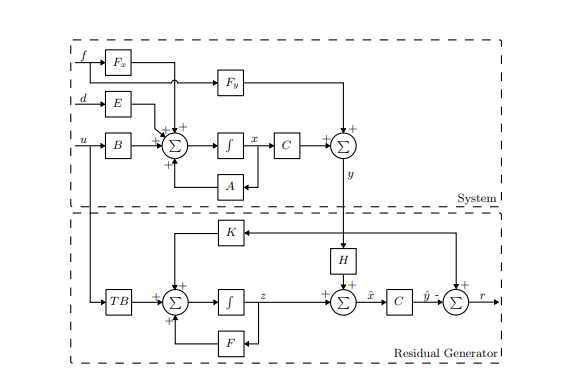
\includegraphics[width=0.7\linewidth]{figures/observer}
	\caption{Observer based residual generator}
	\label{fig:residualobs}
\end{figure}
Moreover, in the \figref{fig:residualobstest} it can be seen how the state error converge asymptotically to zero from the initial conditions along with a change in the attitude of the satellite after 70 seconds, and it can be clearly seen that the disturbance has been decoupled from the residual.
\begin{figure}[H]
	\centering
	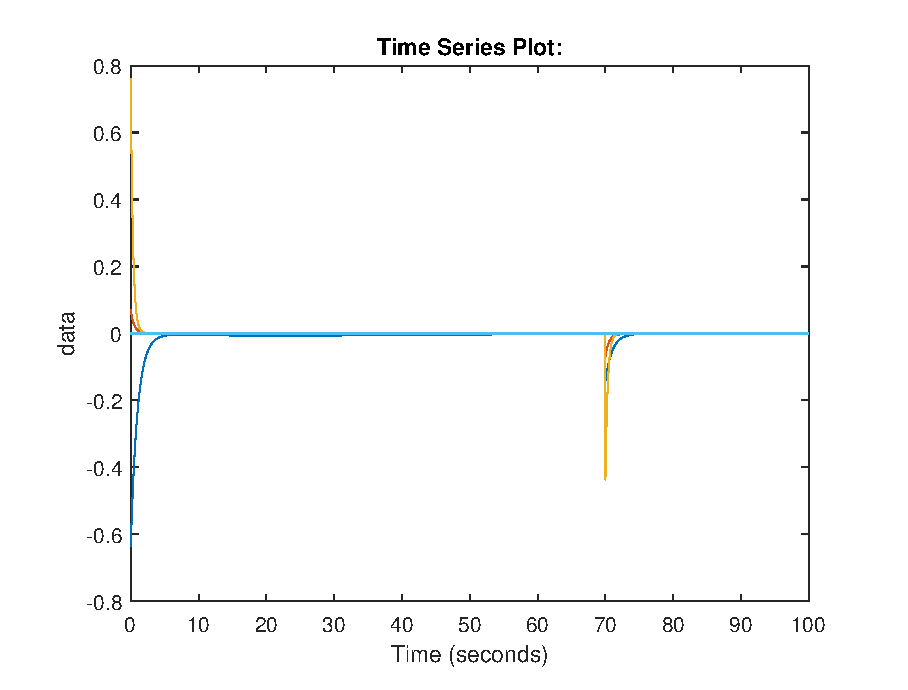
\includegraphics[width=0.7\linewidth]{figures/obstest}
	\caption{Convergence of the state estimation error to zero with the disturbance been decoupled}
	\label{fig:residualobstest}
\end{figure}
The method can be used directly also for the motors. The faults after the detection can be isolated by making the residual sensitive to all but one actuator fault each time, leading to a bank of observers each sensitive to a particular actuator component.
\subsection{CUSUM algorithm and change detection} 